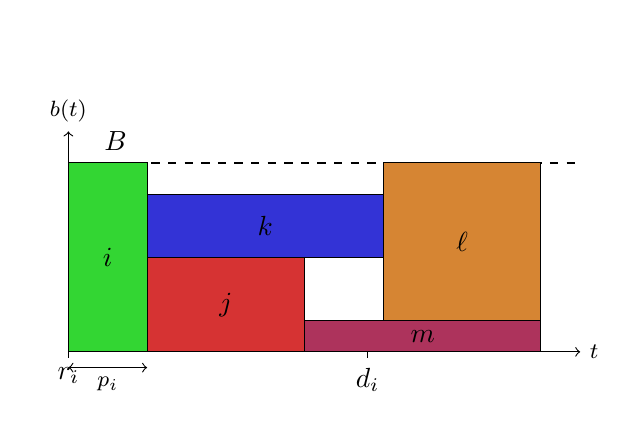
\begin{tikzpicture}
  [yscale=0.4]
  \node at (0,10) {};

  \node[label={[shift={(-0.4,-0.5)}]}] (O) at (0,0) {};
  \draw[fill=red!80!black!80] (1,0) rectangle (3,3)   node[midway] {$j$};
  \draw[dashed,thick] (0,6)   -- (6.5,6);
  \node at (0.6,6.7)  {$B$};
    \draw[<->] (0,-0.5) -- (1,-0.5) node[midway,below] {\footnotesize $p_i$};
    \draw[<->] (0.8,0) -- (0.8,6) node[midway,left] {\footnotesize $b_{i}$};
  
  \draw (0,0) -- (0,-0.2) node[below] {$r_i$};
  \draw (3.8,0) -- (3.8,-0.2) node[below] {$d_i$};
  
  \draw[fill=green!80!black!80] (0,0) rectangle (1,6)   node[midway] {$i$};
  \draw[fill=blue!80!black!80] (1,3) rectangle (4,5)   node[midway] {$k$};
  \draw[fill=orange!80!black!80] (4,1) rectangle (6,6)   node[midway] {$\ell$};
  \draw[fill=purple!80!black!80] (3,0) rectangle (6,1)   node[midway] {$m$};
  \draw[->] (O.center) -- (0,7) node[above] {\footnotesize $b(t)$};
  \draw[->] (O.center) -- (6.5,0) node[right] {\footnotesize $t$};


\end{tikzpicture}
